\en{
Let $ABC$ be a triangle with $AB=AC$ and $\angle BAC=20^\circ$. Let $D$ be the point on the side $AB$ such that $\angle BCD = 70^\circ$. Let $E$ be the point on the side $AC$ such that $\angle CBE = 60^\circ$. Determine the value of the angle $\angle CDE$.

\textbf{Answer:} $\angle CDE=20^\circ$.

\textbf{Solution 1:}
Define $E'$ on the side $AB$ such that $\angle BCE'=60^\circ$, and $X$ the intersection of $BE$ and $CE'$. Straightforward angle chasing gives that $\Delta E'EX$ is equilateral, as it has angles of $60^\circ$. Moreover, $\Delta AE'C$ is isosceles at $E'$, as $\angle E'AC=20^\circ=\angle E'CA$. Consider the reflection preserving this triangle, sending $E'$ to itself, and exchanging $A$ and $C$. Then $D$ and $X$ are also exchanged, as $\angle E'CD=10^\circ=\angle E'AX$, in particular $E'D=E'X$. As $\Delta E'EX$ is equilateral, we can now deduce that $E'D=E'X=E'E$, so that $\Delta DE'E$ is isosceles at $E'$. The rest is angle chasing: 
\[
\angle E'DE=\frac{180^\circ-\angle DE'E}{2}=\frac{180^\circ- 80^\circ}{2}=50^\circ
\]
 and 
\[
\angle CDE= \angle E'DE-\angle E'DC=50^\circ-30^\circ=20^\circ.
\]

\textbf{Solution 2:}
Define $E'$ on the side $AB$ such that $\angle BCE'=60^\circ$, and $E''$ on the side $AC$ such that $\angle BDE''=60^\circ$. Straightforward angle chasing yields $\angle E'DC=30^\circ=\angle E''DC$ and $\angle E'CD=10^\circ=\angle E''CD$, proving that $CD$ is the perpendicular bisector of $E'E''$. As $DE'=DE''$ and $\angle E'DE''= 60^\circ$, $\Delta DE'E''$ is equilateral so that $\angle DE'E''=60^\circ$ and $\angle E''E'E=20^\circ$. This implies that $\angle E''EE'=80^\circ=\angle EE''E'$ so that $\Delta E'' E E'$ is isosceles at $E'$. Looking at side lengths, this implies that $E'D=E'E''=E'E$, so we also have that $\Delta DE'E$ is isosceles at $E'$. We can then conclude like in Solution 1.

\begin{center}
    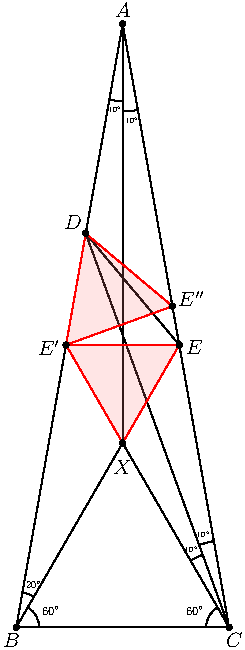
\includegraphics[scale=1]{2021/Final round/MasterSolution/Solutions/f8fig.pdf}
\end{center}

\textbf{Remark :} This drawing has elements from Solutions 1 and 2 : the two constructed equilateral triangles are highlighted.

\newpage
\textbf{Marking scheme - Solution 1} 

\begin{itemize}
    \item 0P: Claiming that $\angle CDE=20^\circ.$
    \item 1P: Introducing $E'$, the point on the side $AB$ such that $\angle E'CB=60^\circ$.
    \item 1P: Showing that $\Delta E'EX$ is equilateral.
    \item 2P: Showing that $E'D=E'X$.
    \item 3P: Conclude.
\end{itemize}

\textbf{Marking scheme - Solution 2} 

\begin{itemize}
    \item 0P: Claiming that $\angle CDE=20^\circ.$
    \item 1P: Introducing $E'$, the point on the side $AB$ such that $\angle E'CB=60^\circ$ and $E''$.
    \item 2P: Showing that $\Delta E'DE''$ is equilateral.
    \item 1P: Showing that $E'E''=E'E$.
    \item 3P: Conclude.
\end{itemize}

}
$0 \le d \le c \le b \le a \le 1 \implies$ \\
$(a+b+c+d)^2(a+2b+3c+4d) \le (a+b+c+d)^3$